\documentclass[a4paper, 12pt]{article}
\usepackage{graphicx}
\usepackage{float}
\graphicspath{{Images/}}
\usepackage{hyperref}
\usepackage{array}
\usepackage{textcomp}
\usepackage{amsmath}
\renewcommand{\arraystretch}{1.07}
\usepackage[utf8]{inputenc}
\hypersetup{
	colorlinks=true,
	linkcolor=red,
	filecolor=blue,      
	urlcolor=cyan,
}

\title{
	Software Engineering 2: PowerEnJoy\\
	\textbf{Project Plan (PP)}\\
	Version 1.0
	\newline
	\begin{figure}[H]
		\centering
		
\includegraphics{polimi_logo}
	\end{figure}
	Politecnico di Milano, A.A. 2016/2017
}
\author{Agosti Isabella, 874835\\Cattivelli Carolina, 879359}
\date{January 22, 2017}
\begin{document}	
	\maketitle
	\tableofcontents
	\section{INTRODUCTION}
\subsection{Purpose}
The purpose of this document is to illustrate in details the concepts expressed in the RASD document, clarifying the architectural choices that have been made and the functionalities that will be developed.
\subsection{Scope}
The system allows registered users to reserve a car via mobile or web application, by letting the system track their position or by inserting a specific address.

A user is considered registered only after filling out a form, receiving a password by the system and logging in for the first time.

The system's main purpose is to protect the environment. For this reason it is based on a car-sharing service using only electric cars.
\newpage 
\subsection{Definitions, Acronyms, Abbreviations} 
\subsubsection{Definitions}
\begin{center}
	\begin{tabular} { | m{4cm} | m{9cm} | }
		\hline
		\textbf{Keyword} & \textbf{Definitions}\\
		\hline
		User & A person that interacts with the PowerEnJoy mobile or web
		application to register to the system.\\
		\hline
		Registered user & A person who already registered to the system, that interacts with the PowerEnJoy mobile or web application in various ways.\\
		\hline
		Employee & A member of the PowerEnJoy staff.\\
		\hline
		Car-sharing service & Model of car rental where people rent cars for short periods of time, often by the hour.\\
		\hline
		Electric car & Automobile that is propelled by one or more electric motors, using electrical energy stored in rechargeable batteries.\\
		\hline
		Registration & The act or process of filling out an online form providing credentials and payment information.\\
		\hline
		Log-in & Process by which a user gains access to the system by identifying and authenticating himself/herself. \\
		\hline
		Reservation & Arrangement through which a registered user holds a car for his use at a later time.\\
		\hline
		Safe area & Area whose position is predefined by the management system. Safe areas are the only ones in which a user is allowed to park a car.\\
		\hline
		Special safe area & Special type of safe area where a car can be recharged.\\
		\hline
		Discount percentage & Discount applied on the user’s last ride only in certain circumstances.\\
		\hline
		Low battery & The car’s battery level is considered ”low” when less than 20\%.\\
		\hline
	\end{tabular}
\end{center}
\newpage
\subsubsection{Acronyms and Abbreviations}
\begin{center}
	\begin{tabular} { | m{5cm} | m{8cm} | }
		\hline
		\textbf{Acronym/abbreviation} & \textbf{Definitions}\\
		\hline
		DB & Database\\
		\hline
		UI & User Interface\\
		\hline
		GUI & Graphical User Interface\\
		\hline
		RASD & Requirements Analysis and Specification Document\\
		\hline
		DD & Design Document\\
		\hline
		UX & User eXperience\\
		\hline
		BCE & Boundary Control Entity\\
		\hline
		UML & Unified Modeling Language\\
		\hline
		AA & Anno Accademico (Academic Year)\\
		\hline
		SOA & Service Oriented Architecture \\
		\hline
		MVC & Model View Controller\\
		\hline
\end{tabular}
\end{center}  

\subsection{Reference Documents}  
\begin{itemize}
	\item Specifications document: Assignments AA 2016-2017.pdf
	\item Sample Design Deliverable Discussed on Nov. 2.pdf
	\item RASD.pdf
\end{itemize} 
\newpage
\subsection{Document Structure}
The document is organized as follows:
\begin{itemize}
	\item \textbf{Introduction}, gives an overview of the design document's contents.
	\item \textbf{Architectural design}:
	\begin{itemize}
		\item \textit{Overview}, describes the high level components and their interaction.
		\item \textit{Component view}, gives a more detailed description of the application's components.
		\item \textit{Deployment view}, presents the components that must be deployed in order for the application to run correctly.
		\item \textit{Runtime view}, describes through sequence diagrams the way components interact to accomplish specific tasks related to our use cases.
		\item \textit{Component interfaces}, presents the interfaces of the application's components.
		\item \textit{Selected architectural styles and patterns}, presents the styles and patterns we used, why and how.  
		\item \textit{Other design decisions}.
	\end{itemize}
	\item \textbf{Algorithm design}, focuses on the definition of the most relevant algorithmic parts.
	\item \textbf{User interface design}, provides an overview on how the  user interface(s) of our system will look like.  
	\item \textbf{Requirements traceability}, explains how the requirements defined in the RASD map to the design elements defined in this document. 
	\item \textbf{Effort spent}, includes information about the number of hours each group member has worked towards the fulfillment of this deadline. 
	\item \textbf{References}, describes the tool used to redact this document and its components.
\end{itemize}
	\section{PROJECT SIZE, COST AND EFFORT ESTIMATION}
This section provides some estimations on the expected size, cost and required effort of the PowerEnJoy project.

For the size estimation part we will use the Function Points approach, considering all the main PowerEnJoy functionalities and estimating the correspondent amount of lines of code to be written in Java. 

For the cost and effort estimation we will instead rely on the COCOMO approach, using as initial guidance the amount of lines of code computed with the FP approach.

\subsection{Size estimation: Function Points}
The Function Points approach provides an estimation of a project size taking as inputs the amount of functionalities to be developed and their complexity.

The complexity is evaluated based on the characteristics of the application and described in the following table:


\subsubsection{Internal Logic Files (ILFs)}

\subsubsection{External Logic Files (ELFs)}

\subsubsection{External Inputs (EIs)} 

\subsubsection{External Inquiries (EQs)}

\subsubsection{External Outputs (EOs)} 

\subsubsection{Overall estimation}

\subsection{Cost and effort estimation: COCOMO II}

\subsubsection{Scale Drivers}

\subsubsection{Cost Drivers}

\subsubsection{Effort equation}

\subsubsection{Schedule estimation}

	\section{SCHEDULE}
In this paragraph we provide our project schedule. 

It is important to notice that, while this project is made for didactic purposes and no implementation and testing will be performed, we have still considered these steps as part of our schedule to take into account what could be the full development of this project, should it continue.

\begin{figure}[H]
	\centering
	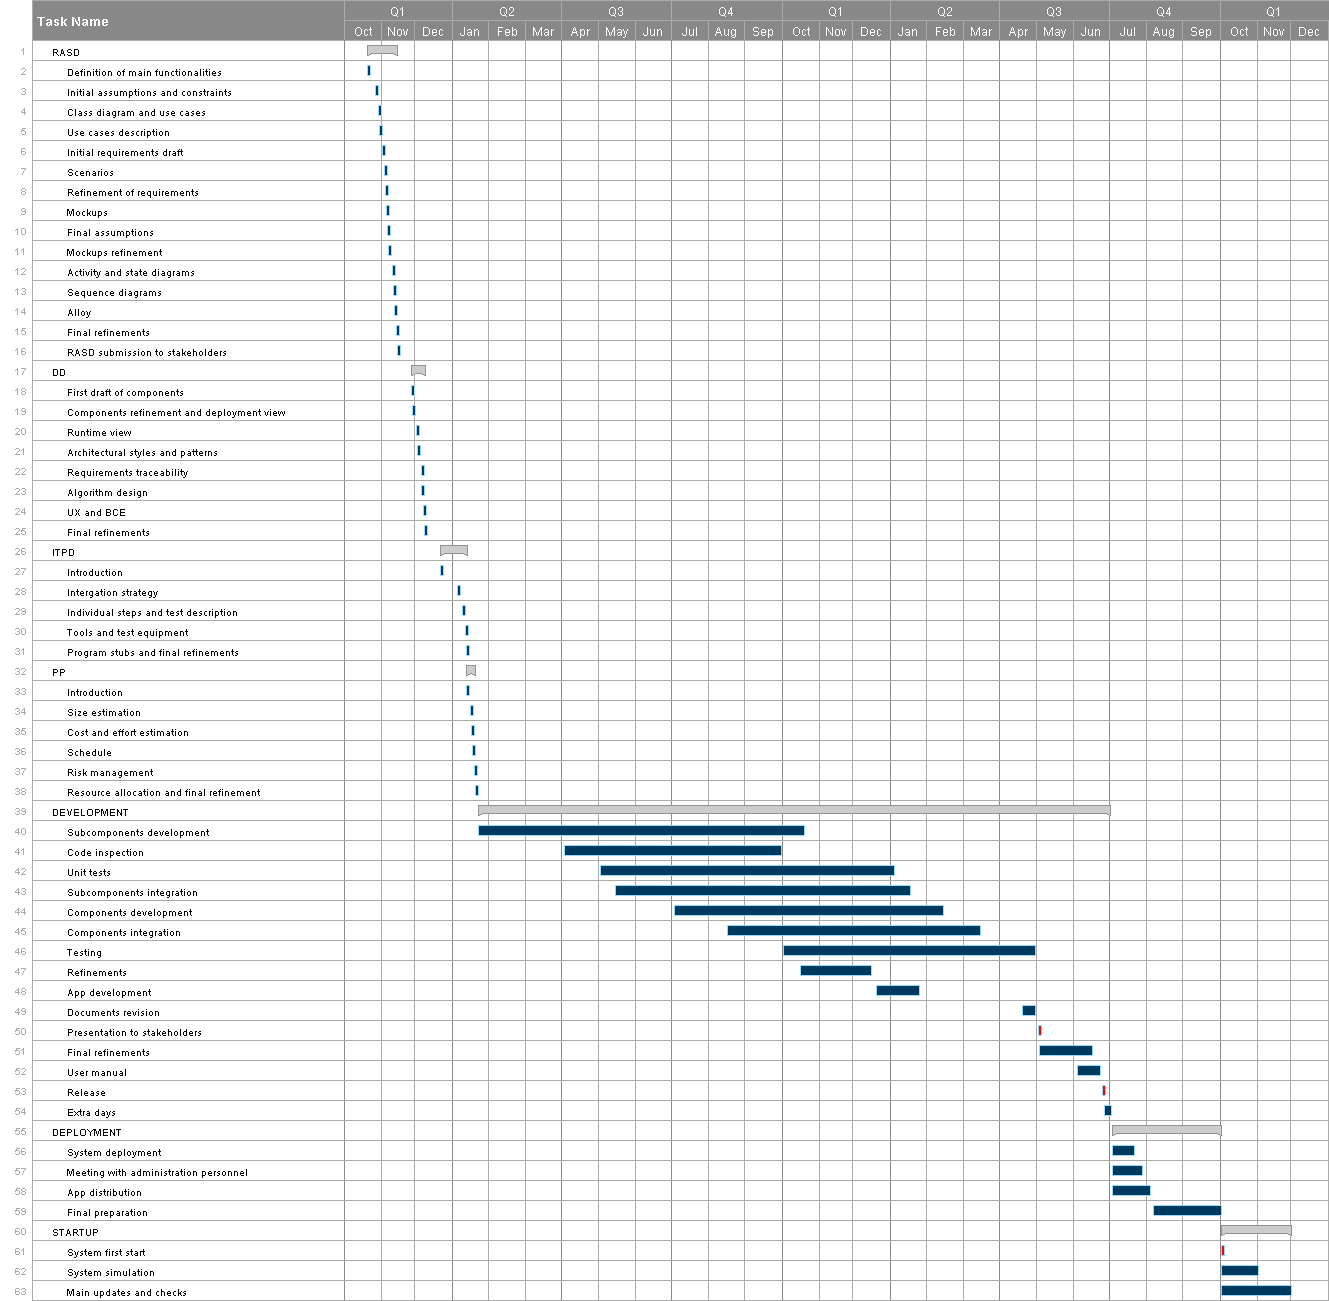
\includegraphics[width=14cm]{Gantt}
\end{figure}

	\section{RESOURCE ALLOCATION}
	\section{RISK MANAGEMENT}
	\section{EFFORT SPENT}
This section includes information about the number of hours each group member has worked towards the fulfillment of this deadline. 

Since we decided to work together every day, the worked hours are going to be the same for each group member. We think this is the best way to achieve good results.  

\subsection{Agosti Isabella}
\begin{itemize}
	\item 13/01/2017: 1h
	\item 16/01/2017: 3h
	\item 17/01/2017: 4h
	\item 18/01/2017: 2h
	\item 19/01/2017: 4h
	\item 20/01/2017: 5h
\end{itemize}
\subsection{Cattivelli Carolina}
\begin{itemize}
	\item 13/01/2017: 1h
	\item 16/01/2017: 3h
	\item 17/01/2017: 4h
	\item 18/01/2017: 2h
	\item 19/01/2017: 4h
	\item 20/01/2017: 5h
\end{itemize}
\end{document}
